\documentclass[11pt]{article}
\usepackage{geometry}
\usepackage{graphicx}
\usepackage{wrapfig}
\usepackage{float}
\usepackage[T1]{fontenc}
\usepackage[utf8]{inputenc}
\usepackage{fixltx2e}
\usepackage{helvet}
\renewcommand{\familydefault}{\sfdefault}
\usepackage{titlesec}
\titlespacing\section{1pt}{12pt plus 2pt minus 2pt}{1pt plus 2pt minus 2pt}
\titlespacing\subsection{1pt}{12pt plus 2pt minus 2pt}{pt plus 2pt minus 2pt}
%\titlespacing\subsubsection{5pt}{12pt plus 2pt minus 2pt}{1pt plus 2pt minus 2pt}
%\usepackage{float}
\usepackage[hidelinks]{hyperref}
\geometry{margin=0.5in}
%opening
\titleformat*{\section}{\small\bfseries}
\title{Investigating the genetic diversity, population structure and demography of Baja and Pacific \emph{Hemisquilla californiensis}}
\bibliographystyle{unsrt}
\date{}
\author{Ethan Holleman}
\begin{document}
\maketitle
\thispagestyle{empty}

\section*{Introduction}


Mantis shrimp are a unique group of carnivorous stomatopods that are believed to have diverged from members of the class \emph{Malacostraca} around 340 million years ago \cite{VanDerWal2017}. Mantis shrimp are notable for both their unique mechanically driven raptorial smashing or spearing claws, which are powerful enough to induce cavitation in the surrounding water \cite{Patek2004, Patek2005} and acutely sensitive visual system which is believed to be the most complex ever discovered in nature \cite{Cronin2014, Milius2012}. Due to their extraordinary physiology, the biology of Mantis shrimp species has been the subject interdisciplinary study by researchers in the fields of optics, material science and biology \cite{Huang2020, Altaqui2021, Donohue2018}. However, comparatively few studies have examined on the genetic structure of Mantis shrimp populations and those that have focused on Asian Mantis shrimp species in the Yellow and East China Seas \cite{Yang2018} where their study is motivated by the greater demand for the shrimp as a specialty seafood in Asian economies. \emph{Hemisquilla californiensis}, the California Mantis shrimp, which ranges from Southern California to Panama \cite{Basch1993BiogeographyOH}, therefore represents a significant gap in population level scientific knowledge of these incredible organisms. \emph{H. californiensis} and other Mantis shrimp species are known to play an important role in marine ecosystems by acting as efficient predators of other crustaceans and oxygenating ocean sediments \cite{Antony2010}. Understanding the genetic history of these crustaceans in their Atlantic range is therefore key for accessing the overall health of important marine ecosystems, such as coral reefs which \emph{H. californiensis} are known to inhabit. 

\begin{wrapfigure}{l}{0.40\textwidth}
	\begin{center}
		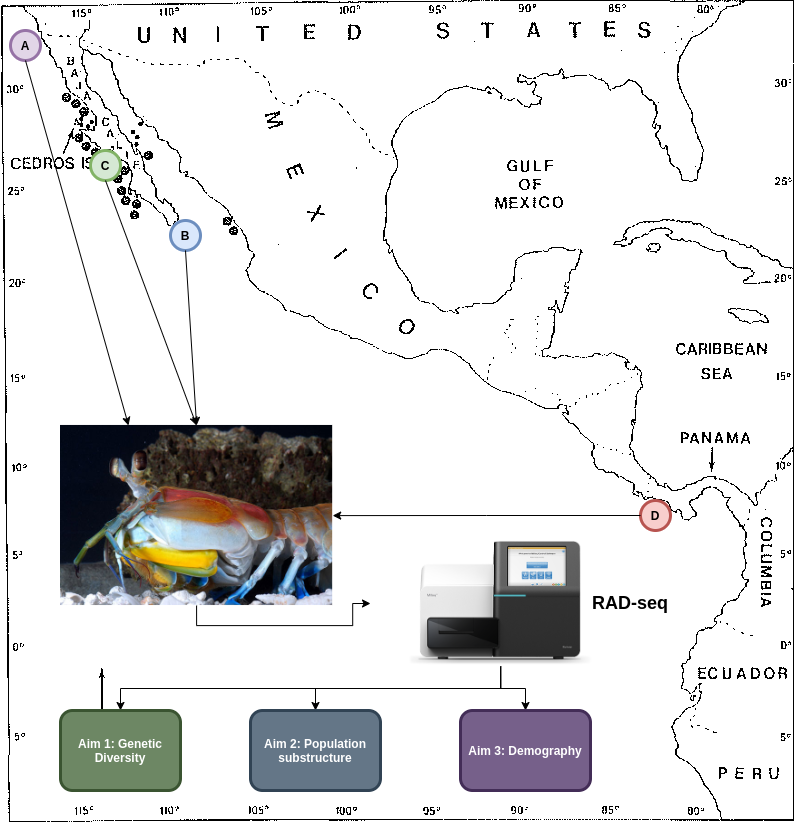
\includegraphics[width=0.35\textwidth]{images/sampling_locations.png}
	\end{center}
	\caption{Proposed \emph{Hemisquilla californiensis} collection locations shown as colored dots. Image adapted from \emph{Basch et al, 93}}
\end{wrapfigure}

Therefore, our main goal is to quantify genetic diversity of \emph{H. californiensis} across their Atlantic range in order to access gene flow between populations and infer effects of recent antropogenic changes to the marine ecosystem by evaluating \emph{H. californiensis} demographic and selective events. Towards this effort we will pursue three specific aims.


\section*{Aim 1: Characterize genetic variation in \emph{H. californiensis} populations.}

Hypothesis: All \emph{H. californiensis} populations will deviate significantly from Hardy-Weinburg equilibrium and correlate with latitude. \emph{H. californiensis} populations are mainly concentrated along the Southern coast of Baja California, with a fewer more Southerly populations identified along the West coast of Panama, although this may be a result of lower resolution reporting \cite{Basch1993BiogeographyOH}. In order to access this we will genotype individuals from 12 Western Baja populations and 2 Western Panamanian populations using restriction site associated DNA sequencing (RAD-seq) \cite{rad2011} which will allow the low-cost genotyping of a large number of individuals. Using RAD-seq data we will identify a number of suitable sites for further genetic analysis based on 
sequence quality metrics. We will also identify sites my mapping RAD-seq reads to homologous regions in the closest high-quality related reference genome; Penaeid shrimp \cite{Zhang2019}. Any calculations made using RAD-seq data ultimately assume that individual reads are independent, an assumption that can be violated by PCR induced bias. To avoid erroneous calculations we will employ protocols that produce random fragment lengths in order to trim PCR duplicates \emph{in silico}. We will then use this trimmed genotype data to calculate allele frequencies for all identified sites across the 14 sampled populations and determine genotypes of each individual using established methods \cite{Rochette2017}. Expected genotype frequencies can then be calculated for each site under the assumptions of Hardy-Weinberg Equilibrium (HWE); random mating and absence of migration between populations, genetic drift and mutation. HHE derived expectations will then be compared to observed genotypes utilizing Chi square tests. This test of significance assumes variables are mutually exclusive; this is appropriate as any two genotypes cannot occur simultaneously. The degree to which each site deviates from HHE expectation can then be compared across each population. 


\section*{Aim 2: Quantify \emph{H. californiensis} population sub-structure to evaluate gene flow}
Hypothesis: \emph{Odontodactylus scyllarus} will show significant gene flow within, but not between, Baja and Panamanian sampling locations. Previous studies examining genetic variation of \emph{Oratosquilla oratoria}, a Mantis shrimp species closely related to the California Mantis shrimp, in the Yellow and East China seas found a surprising degree of gene flow between populations as determined by pairwise F\textsubscript{st} calculations \cite{Yang2018}. This represents occurrence of gene flow at a scale similar to that of the most Northern and Sourthern Baja \emph{H. californiensis} populations but significantly less than distances between Baja and Panamanian populations between which no significant population centers have been identified \cite{Basch1993BiogeographyOH}. However, these studies suffered from lack of high resolution sampling at mid latitudes and therefore gene flow could be occurring if significant numbers of \emph{O. scyllarus} exist along the Western Mexican coast. To answer this question we will utilize the RAD-seq genotype data collected in aim 1 to access gene flow between the 14 sampled populations through pairwise comparison of inbreeding F statistics, and through a Bayesian approach to sub-population assignment. First, we will determine reductions in heterozygosity due to genetic differentiation between the sampled populations by calculating the pairwise F\textsubscript{st} values between the 14 sampled populations. Ultimately, F\textsubscript{st} is evaluated against the expected heterozygosity of the sub-populations if they were merged, had equal size and were randomly mating. We will evaluate error in our estimations through permutation testing, which repeatedly randomly assigns individuals to a sub-population and evaluates  F\textsubscript{st} to ultimately create a probability distribution which can then be used to evaluate the significance of our actual results. We expect pairwise F\textsubscript{st} to deviate significantly from expectation between proximal Baja populations but to be non-significant for all pairwise comparisons that include the Panamanian populations. Additionally, using the pairwise F\textsubscript{st} calculations between Baja populations, we will determine the mean decrease in F\textsubscript{st} per unit distance between populations. If no major \emph{O. scyllarus} exist between the Baja and Panamanian regions, this expectation should be predictive of the degree of decrease in pairwise F\textsubscript{st} between Baja and Panamanian populations. A decrease that is significantly less than this expectation would indicate greater gene flow between these populations than would be expected, indicating the presence of mid-latitude \emph{H. californiensis} populations. This however assumes that geographic distance is the main determinant of gene flow in \emph{H. californiensis} which is reasonable considering their relatively stationary lifestyle \cite{Reaka1980}. Next, we will also preform an admixture analysis in order to estimate the proportion of ancestry from each subpopulation for all individuals. Similarly to pairwise  F\textsubscript{st} analysis we expect to find that significant admixture between but not within Baja and Panamanian populations. While out analysis will consider ancestry from multiple populations it ultimately relies on the same assumptions made under two-population maximum likelihood admixture model. Namely, that all sites are independent (not experiencing linkage disequilibrium) and mutually exclusive. We will quantify error in our estimations by calculating 95\% confidence interval derived from maximum likelihood distributions that consider $\theta$ (percent ancestry) in steps of 0.01. Finally, we will visually evaluate sub-population structure using principal component analysis of all genotyped sites. We expect to find significant separation between Baja and Panamanian populations with some, but lower degree of sub-clustering of Baja populations that is reflects geographic separation. 


\section*{Aim 3: Determine demographic history between Northern and Southern California Mantis shrimp populations.}

Hypothesis: \emph{H. californiensis} has undergone a recent global decrease in population size across its range in the last 200 years. It is estimated that ocean pH levels have decreased approximately 30\% in the last 200 years \cite{noauthor_ocean_nodate}. This has been shown to be especially detrimental to species that rely on an calcium based exoskeleton, such as crustaceans including \emph{H. californiensis} \cite{Taylor2015}. In order to access if recent decreases in ocean pH have impacted \emph{H. californiensis} we will utilize approximate Bayesian computation (ABC) to infer both the most likely timing and magnitude of a potential population decrease based on allele frequency data generated in the course of aim 1. Since we expect an overall decline in \emph{H. californiensis} populations but lack significant data regarding their population history we will utilize a bounded uniform prior which assumes equal probability of all parameters, time and strength of decline, within a discrete range. Our parameter space will be bounded between 10 and 50,000 generations in time and between a 0 and 100 fold change in population size (strength of decline). This will allow for consideration of both recent (anthropogenic ocean acidification) and historical demographic events. The most probable parameters to explain \emph{H. californiensis} observed allele frequency spectrum will be identified by measuring euclidean distances to the simulated allele frequency spectra. Due to how recently ocean acidification has occurred, we would not expect significant selection to have occurred. This would lead to changes in the allele frequency spectrum at specific loci opposed to genome wide changes expected by a demographic event. We will therefore compare the allele frequency spectrum of specific loci to genome-wide background to validate acidification as a demographic level perturbation. Finally, we will compare ABC results across all sampled populations. Since ocean acidification should effect all \emph{H. californiensis} populations similarly, we would not expect to see significantly differentiated time and strength of selection parameters across populations. Finally, to directly connect our population level results to \emph{H. californiensis} physiology, during sample collection we will measure calcium content of exoskeletons from a select number of individuals from all populations using Inductivity Coupled Plasma-Optical Emission Spectrometry Instruments (ICP-OES) and compare to measurements from historical Mantis shrimp samples. We expect to observe an overall decrease in calcium content.  

\pagebreak

\bibliography{refs}

\end{document}
